% RICHARD DAVIES
% UK FIRM DYNAMICS 
% PAPER, FEBRUARY 2022

%------------------------------------------------------------
%------------------------------------------------------------
%Setting up the document

\documentclass{beamer}
\usepackage[utf8]{inputenc}

\usetheme{Madrid}
\usecolortheme{default}
\useinnertheme{circles}

\definecolor{Logo1}{RGB}{18, 43, 57}
\definecolor{Logo2}{RGB}{54, 183, 180}
\definecolor{Logo3}{RGB}{23, 159, 219}

\setbeamercolor*{palette primary}{bg=Logo1, fg=white}
\setbeamercolor*{palette secondary}{bg=Logo2, fg=white}
\setbeamercolor*{palette tertiary}{bg=Logo3, fg=Logo1}
\setbeamercolor*{palette quaternary}{bg=Logo1,fg=white}
\setbeamercolor{structure}{fg=Logo1} % itemize, enumerate, etc
\setbeamercolor{section in toc}{fg=Logo1} % TOC sections

%------------------------------------------------------------
%------------------------------------------------------------
%This block of code defines the information to appear in the
%Title page
\title[UK productivity] %optional
{The UK productivity puzzle}

\subtitle{Declining firm dynamism}

\author[Richard Davies] % (optional)
{Richard Davies}

\institute[] % (optional)
{
  Economics Observatory\\
  U Bristol and CEP
}

\date[Declining dynamism] % (optional)
{POID presentation, February 2022}


%\logo{\includegraphics[height=.5cm]{logo-footer.png}}

%End of title page configuration block
%------------------------------------------------------------



%------------------------------------------------------------
%The next block of commands puts the table of contents at the 
%beginning of each section and highlights the current section:

\AtBeginSection[]
{
  \begin{frame}
    \frametitle{Overview}
    \tableofcontents[currentsection]
  \end{frame}
}
%------------------------------------------------------------


\begin{document}

%The next statement creates the title page.
\frame{\titlepage}


%---------------------------------------------------------
%This block of code is for the table of contents after
%the title page
\begin{frame}
\frametitle{Overview}
\tableofcontents
\end{frame}
%---------------------------------------------------------


%---------------------------------------------------------
%---------------------------------------------------------
% FIRST SECTION

\section{Motivation: the two puzzles}


%---------------------------------------------------------
%---------------------------------------------------------
% Slide 1 - productivity puzzle - THE OLD PUZZLE
\begin{frame}
\frametitle{The UK productivity puzzle I}

\begin{figure}
%\caption{Caption for figure}
%\label{Graph1}
\centering
\includegraphics[width=0.75\textwidth]{ukGermany.PNG}
\end{figure}

\href{https://cep.lse.ac.uk/pubs/download/special/cepsp34.pdf}{\beamergotobutton{Bernick, Davies, Valero (2017)}}

\end{frame}
%---------------------------------------------------------
%---------------------------------------------------------

%---------------------------------------------------------
%---------------------------------------------------------
% Slide 2 - productivity puzzle - THE OLD PUZZLE
\begin{frame}
\frametitle{The UK productivity puzzle I}

The history of a British obsession:
\vspace{0.3cm}
 
\begin{itemize}
\item 1929. Macmillan Committee [Keynes]
\item 1942-1965. National Production Advisory Council
\item 1957. Council on Prices, Productivity and Incomes. [Cohen]
\item 1960s. "Declinist" literature
\item 1962-1992. National Economic Development Council (NEDC) 
\end{itemize}

\vspace{0.3cm}
Principal concerns the "gap" between the UK and US, Germany.
\vspace{0.3cm}


\end{frame}
%---------------------------------------------------------
%---------------------------------------------------------


%---------------------------------------------------------
%---------------------------------------------------------
% Slide 6 - Stylised Facts 1
\begin{frame}
\frametitle{Minding the Gap}

\begin{columns}

\column{0.5\textwidth}

\begin{figure}
%\caption{Caption for figure}
%\label{Graph1}
\centering
\includegraphics[width=1\textwidth]{chart_ProdGap.PNG}
\end{figure}

\column{0.5\textwidth}

\begin{itemize}
\item Gap between the US and UK became a concern in the 1940s.
\item Since the 1970s has been stable. 
\item Compared to G7 countries the UK is mid-tier. Better than 50 years ago.
\item Note: Italy... 

\item \href{https://www.rapidcharts.io/productivity}{\beamergotobutton{Live chart}}
\end{itemize}



\end{columns}
\end{frame}
%---------------------------------------------------------
%---------------------------------------------------------


%---------------------------------------------------------
%---------------------------------------------------------
% Slide 6 - Stylised Facts 1
\begin{frame}
\frametitle{Minding the Gap II}

\begin{columns}

\column{0.5\textwidth}

\begin{figure}
%\caption{Caption for figure}
%\label{Graph1}
\centering
\includegraphics[width=1\textwidth]{chart_ProdGap_OECD.JPG}
\end{figure}

\column{0.5\textwidth}

\begin{itemize}
\item Same chart but for a wider group - the OECD.
\item UK is again mid-tier.
\item Note: Ireland... 

\item \href{https://www.rapidcharts.io/productivity}{\beamergotobutton{Live chart}}
\end{itemize}



\end{columns}
\end{frame}
%---------------------------------------------------------
%---------------------------------------------------------



%---------------------------------------------------------
%---------------------------------------------------------
% Slide 3 - productivity puzzle - time series
\begin{frame}
\frametitle{The UK productivity puzzle}

\begin{figure}
%\caption{Caption for figure}
%\label{Graph1}
\centering
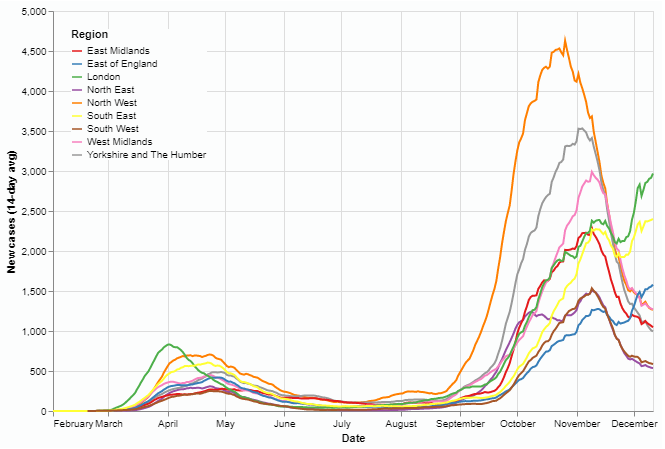
\includegraphics[width=0.5\textwidth]{chart1.PNG}
\end{figure}

\href{https://www.rapidcharts.io/productivity}{\beamergotobutton{Live and interactive chart}}

\end{frame}
%---------------------------------------------------------
%---------------------------------------------------------


%---------------------------------------------------------
%---------------------------------------------------------
% Slide 6 - Stylised Facts 1
\begin{frame}
\frametitle{The puzzle - macro data}

\begin{columns}

\column{0.5\textwidth}

\begin{figure}
%\caption{Caption for figure}
%\label{Graph1}
\centering
\includegraphics[width=1\textwidth]{chart3.png}
\end{figure}

\column{0.5\textwidth}

\begin{itemize}
\item Slowdown in GVA expansion.


\end{itemize}
\end{columns}
\end{frame}
%---------------------------------------------------------
%---------------------------------------------------------






%---------------------------------------------------------
%---------------------------------------------------------
% Slide 6 - Stylised Facts 1
\begin{frame}
\frametitle{The puzzle - macro data}

\begin{columns}

\column{0.5\textwidth}

\begin{figure}
%\caption{Caption for figure}
%\label{Graph1}
\centering
\includegraphics[width=1\textwidth]{chart2.png}
\end{figure}

\column{0.5\textwidth}

\begin{itemize}
\item Job-rich recovery from GFC.


\end{itemize}
\end{columns}
\end{frame}
%---------------------------------------------------------
%---------------------------------------------------------




%---------------------------------------------------------
%---------------------------------------------------------
% Slide 6 - Stylised Facts 1
\begin{frame}
\frametitle{Candidate explanations - macro data}

\begin{columns}

\column{0.5\textwidth}

\begin{figure}
%\caption{Caption for figure}
%\label{Graph1}
\centering
\includegraphics[width=1\textwidth]{chart4.png}
\end{figure}

\column{0.5\textwidth}

\begin{itemize}
\item Slowdown in GVA expansion.


\end{itemize}
\end{columns}
\end{frame}
%---------------------------------------------------------
%---------------------------------------------------------


%---------------------------------------------------------
%---------------------------------------------------------
% Slide 6 - Stylised Facts 1
\begin{frame}
\frametitle{Candidate explanations - macro data}

\begin{columns}

\column{0.5\textwidth}

\begin{figure}
%\caption{Caption for figure}
%\label{Graph1}
\centering
\includegraphics[width=1\textwidth]{chart5.png}
\end{figure}

\column{0.5\textwidth}

\begin{itemize}
\item Slowdown in GVA expansion.


\end{itemize}
\end{columns}
\end{frame}
%---------------------------------------------------------
%---------------------------------------------------------



%---------------------------------------------------------
%---------------------------------------------------------
% Slide 6 - Stylised Facts 1
\begin{frame}
\frametitle{Candidate explanations - macro data}

\begin{columns}

\column{0.5\textwidth}

\begin{figure}
%\caption{Caption for figure}
%\label{Graph1}
\centering
\includegraphics[width=1\textwidth]{chart6.png}
\end{figure}

\column{0.5\textwidth}

\begin{itemize}
\item Slowdown in GVA expansion.


\end{itemize}
\end{columns}
\end{frame}
%---------------------------------------------------------
%---------------------------------------------------------


%---------------------------------------------------------
%---------------------------------------------------------
% Slide 3 - productivity facts
\begin{frame}
\frametitle{Summing up}

\begin{itemize}
    \item<1-> Output per hour grew 2.4\% per year between 1971 and 2007.
    \item<2-> Since then it has grown by just 0.3\% per year. 
    \item<3-> The "gap" literature has various culprits for this. Low investment, low R&D, slow software adoption. None of these seem to show the familiar kink. 
    \item<4-> Can micro data help?
\end{itemize}

\end{frame}
%---------------------------------------------------------
%---------------------------------------------------------


%---------------------------------------------------------
%---------------------------------------------------------
% Slide 3 - productivity puzzle - time series
\begin{frame}
\frametitle{The puzzle - micro data edition}

\begin{figure}
%\caption{Caption for figure}
%\label{Graph1}
\centering
\includegraphics[width=0.5\textwidth]{chart7.PNG}
\end{figure}

\href{https://www.rapidcharts.io/productivity}{\beamergotobutton{Live and interactive chart}}

\end{frame}
%---------------------------------------------------------
%---------------------------------------------------------




%---------------------------------------------------------
%---------------------------------------------------------
% SECTION 2 - OVERVIEW OF PAPER

\section{Paper Overview}


%---------------------------------------------------------
%---------------------------------------------------------
% Slide 5 - This paper
\begin{frame}
\frametitle{This paper}

\begin{itemize}
    \item Use firm-level data for the population of UK firms, taken from the BSD. XYZ observations for XYZ firms. 
    \item Construct descriptive statistics on business dynamics: birth rate, death rate, entry, age. Compare these with US literature.  
    \item Produce new facts on job reallocation. 
    \item Estimate simple model of firm responsiveness. This has declined in the UK. 
    \item Argue that reallocation may be an overlooked problem in the UK.
\end{itemize}

\end{frame}
%---------------------------------------------------------
%---------------------------------------------------------


%---------------------------------------------------------
%---------------------------------------------------------
% SECTION 3 - DATA AND STYLISED FACTS

\section{Data and facts on business demographics}


%---------------------------------------------------------
%---------------------------------------------------------
% Slide 5 - This paper
\begin{frame}
\frametitle{Data I - the BSD}

\begin{itemize}
    \item Business Structure Database (BSD), 1997-2020
    \item Population of firms, included based on tax criteria.
    \item VAT threshold (£85,000) and/or registered for PAYE.
    \item Will exclude smallest sole-proprietor firms.
    
\end{itemize}

\end{frame}
%---------------------------------------------------------
%---------------------------------------------------------


%---------------------------------------------------------
%---------------------------------------------------------
% Slide 5 - This paper
\begin{frame}
\frametitle{Data II - preparing panel}

\begin{itemize}
    \item Raw data is ~ 70m.
    \item I drop financial industries, public sector, health, education.
    \item Also drop firms with 0 employment (but not 0 turnover).
    \item Exclude firms who change SIC.
    \item Refer to this as "Market Economy". ~ 49 million observations.
    
\end{itemize}

\end{frame}
%---------------------------------------------------------
%---------------------------------------------------------


%---------------------------------------------------------
%---------------------------------------------------------
% Slide 5 - This paper
\begin{frame}
\frametitle{Data III - the panel}

\begin{itemize}
    \item Final dataset has 7.8m firms.
    \item 4.9m of these are present for 5 years or less.
    \item 332k are present in every year. 
    \item The median UK firm is tiny. 4m have just 1 employee. 6.9m have 5 or fewer employees.
    
\end{itemize}

\end{frame}
%---------------------------------------------------------
%---------------------------------------------------------



%---------------------------------------------------------
%---------------------------------------------------------
% Slide - Stylised Facts 1
\begin{frame}
\frametitle{The puzzle: micro data version}

\begin{columns}

\column{0.5\textwidth}

\begin{figure}
%\caption{Caption for figure}
%\label{Graph1}
\centering
\includegraphics[width=1\textwidth]{chart7.png}
\end{figure}

\column{0.5\textwidth}

\begin{itemize}
\item Macro puzzle set out as output per hour (GVA/hours worked)
\item BSD variables are revenue and employment.
\item Puzzle still exists when using revenue-labour productivity:
    \item 2001-2010: RLP rose 54\%
    \item 2010-2019: RLP rose 9\%
\item Cumulative gap is XX\%
\item \href{https://www.rapidcharts.io/productivity}{\beamergotobutton{Live chart}}
\end{itemize}



\end{columns}
\end{frame}
%---------------------------------------------------------
%---------------------------------------------------------




%---------------------------------------------------------
%---------------------------------------------------------
% Slide - Stylised Facts 1
\begin{frame}
\frametitle{Stylised facts: a laundry list}

Quick stock take:

\begin{itemize}
\item Two puzzles: the gap and the kink.
\item The kink also exists in micro data using RLP. 
\end{itemize}

Next step - look at simple stylised facts for clues:

\begin{itemize}
\item Births and deaths.
\item Age at death, age structure. 
\item Young firms' shares.
\item Cohort effects
\item Foreign ownership

\end{itemize}

Suggestions for other metrics welcome....



\end{frame}
%---------------------------------------------------------
%---------------------------------------------------------



%---------------------------------------------------------
%---------------------------------------------------------
% Slide - Stylised Facts 2
\begin{frame}
\frametitle{Births and deaths}

\begin{columns}

\column{0.5\textwidth}

\begin{figure}
%\caption{Caption for figure}
%\label{Graph1}
\centering
\includegraphics[width=1\textwidth]{chart8.png}
\end{figure}

\column{0.5\textwidth}

\begin{itemize}
\item Births and deaths move but no clear time trend.
\item Both average around 10\%.
\item Common trend and level among industries.
\item Exception: hospitality - birth and death rates ~ 20\%.
\item \href{https://www.rapidcharts.io/productivity}{\beamergotobutton{Live chart}}
\end{itemize}


\end{columns}
\end{frame}
%---------------------------------------------------------
%---------------------------------------------------------


%---------------------------------------------------------
%---------------------------------------------------------
% Slide - Stylised Facts 2
\begin{frame}
\frametitle{Births - industries}





\begin{figure}
%\caption{Caption for figure}
%\label{Graph1}
\centering
\includegraphics[width=.7\textwidth]{chart10.png}
\end{figure}


\end{frame}
%---------------------------------------------------------
%---------------------------------------------------------


%---------------------------------------------------------
%---------------------------------------------------------
% Slide - Stylised Facts 3
\begin{frame}
\frametitle{Age at death}

\begin{columns}

\column{0.5\textwidth}

\begin{figure}
%\caption{Caption for figure}
%\label{Graph1}
\centering
\includegraphics[width=1\textwidth]{chart_placeholder.png}
\end{figure}

\column{0.5\textwidth}

\begin{itemize}
\item Probability of death falls with age.
\item In a given year, most deaths (~60\%) are firms <5y old.
\item \href{https://www.rapidcharts.io/productivity}{\beamergotobutton{Live chart}}
\end{itemize}


\end{columns}
\end{frame}
%---------------------------------------------------------
%---------------------------------------------------------


%---------------------------------------------------------
%---------------------------------------------------------
% Slide - Stylised Facts 4
\begin{frame}
\frametitle{Young firms shares}

\begin{columns}

\column{0.5\textwidth}

\begin{figure}
%\caption{Caption for figure}
%\label{Graph1}
\centering
\includegraphics[width=1\textwidth]{chart_placeholder.png}
\end{figure}

\column{0.5\textwidth}

\begin{itemize}
\item US literature: young firms shares falling.
\item UK. Young firms share of total employment stable.
\item UK. Young firms share of total revenue falling.
\item Striking reductions in some industries:
\item Manufacturing: 6\% $\rightarrow$ 4\% 
\item Retail: 8\% $\rightarrow$ 6\% 
\item Wholesale: 10\% $\rightarrow$ 5\%
\item IT: 30\% $\rightarrow$ 10\%

\item \href{https://www.rapidcharts.io/productivity}{\beamergotobutton{Live chart}}
\end{itemize}


\end{columns}
\end{frame}
%---------------------------------------------------------
%---------------------------------------------------------


%---------------------------------------------------------
%---------------------------------------------------------
% Slide - Stylised Facts 5
\begin{frame}
\frametitle{Age structure}

\begin{columns}

\column{0.5\textwidth}

\begin{figure}
%\caption{Caption for figure}
%\label{Graph1}
\centering
\includegraphics[width=1\textwidth]{chart9.png}
\end{figure}

\column{0.5\textwidth}

\begin{itemize}
\item Firms are getting older:
\item Central age (~median): 7 $\rightarrow$ 7 
\item Mean age:  9 $\rightarrow$ 13 
\item Revenue weighted age: 13 $\rightarrow$ 26

\item \href{https://www.rapidcharts.io/productivity}{\beamergotobutton{Live chart}}
\end{itemize}


\end{columns}
\end{frame}
%---------------------------------------------------------
%---------------------------------------------------------


%---------------------------------------------------------
%---------------------------------------------------------
% Slide - Stylised Facts 6
\begin{frame}
\frametitle{Cohort effects}

\begin{columns}

\column{0.5\textwidth}

\begin{figure}
%\caption{Caption for figure}
%\label{Graph1}
\centering
\includegraphics[width=1\textwidth]{chart13.png}
\end{figure}

\column{0.5\textwidth}

\begin{itemize}
\item The GFC affected cohorts:
\item E.g. 2005 vs 2010 cohort, revenue share at age 3, 2\% vs 1\%.

\item \href{https://www.rapidcharts.io/productivity}{\beamergotobutton{Live chart}}
\end{itemize}


\end{columns}
\end{frame}
%---------------------------------------------------------
%---------------------------------------------------------

%---------------------------------------------------------
%---------------------------------------------------------
% Slide - Re-allocation 1
\begin{frame}
\frametitle{Size and productivity}


\begin{figure}
%\caption{Caption for figure}
%\label{Graph1}
\centering
\includegraphics[width=0.8\textwidth]{chart14.jpg}
\end{figure}

\end{frame}
%---------------------------------------------------------
%---------------------------------------------------------


%---------------------------------------------------------
%---------------------------------------------------------
% Slide - Re-allocation 1
\begin{frame}
\frametitle{A lost decade: the median UK firm}


\begin{figure}
%\caption{Caption for figure}
%\label{Graph1}
\centering
\includegraphics[width=0.8\textwidth]{chart15.jpg}
\end{figure}

\end{frame}
%---------------------------------------------------------
%---------------------------------------------------------






\section{Job reallocation}


%---------------------------------------------------------
%---------------------------------------------------------
% Slide - Stylised Facts 1
\begin{frame}
\frametitle{Reallocation}

Measure reallocation as:

\begin{itemize}
\item Enter
\item Grow
\item Shrink
\item Exit
\end{itemize}

\begin{itemize}
\item Reallocation falling in the US.
\item Is it in the UK?
\item Is micro level reallocation important for aggregate productivity?

\end{itemize}

\end{frame}
%---------------------------------------------------------
%---------------------------------------------------------



%---------------------------------------------------------
%---------------------------------------------------------
% Slide - Re-allocation 1
\begin{frame}
\frametitle{Who hires and fires?}


\begin{figure}
%\caption{Caption for figure}
%\label{Graph1}
\centering
\includegraphics[width=0.8\textwidth]{chart11.png}
\end{figure}

\end{frame}
%---------------------------------------------------------
%---------------------------------------------------------


%---------------------------------------------------------
%---------------------------------------------------------
% Slide - Re-allocation 1
\begin{frame}
\frametitle{Dormant firms}

Some firms seem committed to never change size.


\end{frame}
%---------------------------------------------------------
%---------------------------------------------------------


%---------------------------------------------------------
%---------------------------------------------------------
% Slide - Re-allocation 1
\begin{frame}
\frametitle{UK reallocation - micro data}


\begin{figure}
%\caption{Caption for figure}
%\label{Graph1}
\centering
\includegraphics[width=0.8\textwidth]{chart16.png}
\end{figure}

\end{frame}
%---------------------------------------------------------
%---------------------------------------------------------

%---------------------------------------------------------
%---------------------------------------------------------
% Slide - Re-allocation 1
\begin{frame}
\frametitle{UK reallocation - micro data}


\begin{figure}
%\caption{Caption for figure}
%\label{Graph1}
\centering
\includegraphics[width=0.8\textwidth]{chart18.jpg}
\end{figure}

\end{frame}
%---------------------------------------------------------
%---------------------------------------------------------



%---------------------------------------------------------
%---------------------------------------------------------
% Slide - Stylised Facts 1
\begin{frame}
\frametitle{The missing reallocation}

The missing reallcation is worth £2.4 trillion.

\begin{itemize}
\item x
\item x
\item x
\item x
\end{itemize}


\end{frame}
%---------------------------------------------------------
%---------------------------------------------------------


\section{Shocks vs Responsiveness}

\section{Simple model + counterfactual}



%---------------------------------------------------------
%Highlighting text
\begin{frame}
\frametitle{Ongoing work}

This is work in \alert{progress} please send any comments or questions.

\begin{block}{Plan}
Set out the plan
\end{block}

\begin{alertblock}{Problems}
Set out main problems
\end{alertblock}

\begin{examples}{Economy 2030}
Set out the findings for the Economy 2030 project.
\end{examples}
\end{frame}
%---------------------------------------------------------


\end{document}